\section{Testing}
\enumstart
	\item Why does Software contain bugs?
	\enumstart
		\item Ability to predict the behaviour of complex software is limited
		\item We make mistakes
		\enumstart
			\item Unclear requirements, miscommunication
			\item Wrong assumptions
			\item Design errors
			\item Coding errors
		\enumend
	\enumend
	\item Increasing software reliability
	\enumstart
		\item Fault avoidance
		\enumstart
			\item Statically - without executing the program
			\item Developement methodologies
		\enumend
		\item Fault detection
		\enumstart
			\item Dynamically - executing the program
			\item Static code checkers
		\enumend
		\item Fault tolerance
		\enumstart
			\item Recover from faults at runtime
		\enumend
	\enumend
	\item Error
	\enumstart
		\item Deviation of the observed behaviour from the required behaviour
		\item Functional
		\item Non-functional
	\enumend
	\item Testing
	\enumstart
		\item Process of executing a program to find errors
		\item Testing can only show the presence of bugs, not their absence
	\enumend
	\item Test harness - Collection of software and test data to automate test execution
	\\ 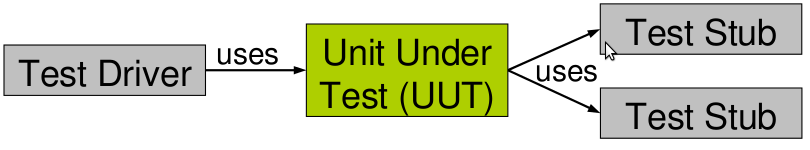
\includegraphics[width=0.5\textwidth]{img/test_harness.png}
	\enumstart
		\item Test driver - Applies test cases to UUT, including setup and cleanup
		\item Test stub - partial implementation that simulates the missing component by returning fake data
	\enumend
\enumend

\subsection{Unit testing}
\enumstart
	\item Testing of individual subsystems
	\item Goal: confirm that subsystem is correctly implemented and carries out the intended functionality
	\item To increase test coverage, test each method with several inputs
	\enumstart
		\item Cover valid and invalid inputs
		\item Cover different paths through the method
	\enumend
	\item Parameterized unit tests
	\enumstart
		\item Decouple test driver from test data
		\item Test data can be specified as values, ranges or random values
		\item Requires generic test oracles
	\enumend
	\item Rules
	\enumstart
		\item All tests should be fully automatic and check their own results
		\item Run tests frequently
		\item For each bug, write a unit test that exposes the bug
		\item Concentrate your tests on boundary conditions
		\item Test if exceptions are raised when things are expected to go wrong
		\item Better to write and run incomplete tests, than to not run tests at all
	\enumend
\enumend

\subsection{Integration testing}
\enumstart
	\item Testing of groups of subsystems
	\item Motivation: many faults result from the interaction of subsystems
	\item Goal: Test interfaces between subsystems
	\item Important: Unit test all classes in the subsystem before integration testing
	\item Strategies
	\enumstart
		\item Order in which the subsystems are selected for testing and integration
		\item Big-bang (non-incremental)
		\item Bottom-up
		\item Top-down
		\item Sandwich testing
		\item Continuous integration
	\enumend
\enumend

\subsection{System testing}
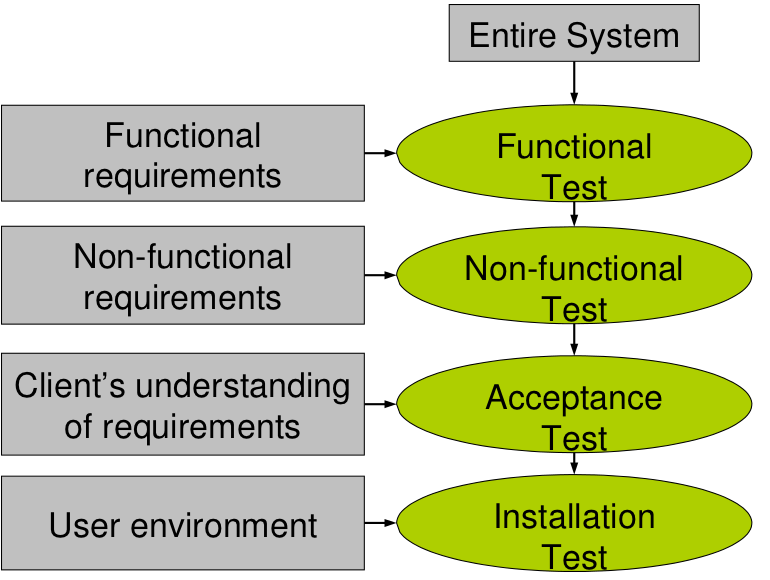
\includegraphics[width=0.5\textwidth]{img/system_testing.png}

\subsubsection{Functional testing}
\enumstart
	\item Testing functionality
	\item Treat system as a black box
	\item Test cases describe
	\enumstart
		\item Input data
		\item Flow of events
		\item Results to check
	\enumend
\enumend

\subsubsection{Non-functional testing}
\enumstart
	\item Stress testing (Explore limits of the system)
	\item Volume testing (Large amounts of data)
	\item Configuration testing (Various software and hardware configurations)
	\item Compatibility testing (e.g. backward compatibility)
	\item Security testing
	\item Timing testing
	\item Environmental testing (tolerance for heat, humidity, $\mathellipsis$)
	\item Recovery testing
	\item Usability testing
\enumend

\subsubsection{Acceptance testing}
\enumstart
	\item Demonstrate to customer
	\item Choice of test is made by clients
	\item Performed by the client
	\item Alpha-test / Beta-test
\enumend

\subsubsection{Installation testing}
\enumstart
	\item Test what users will do to install and set up the software
	\item Different environments
	\item Different configurations
\enumend

\subsubsection{Testing strategies}
\enumstart
	\item Exhaustive testing
	\item Random testing
	\item Functional-/black box testing
	\item Structural-/white box testing
\enumend

\subsection{Functional testing}
\enumstart
	\item Test suite should be complete w.r.t specification
	\item Test suite should be as precise as possible
	\item Treat the program as a black box
	\item Use functional specification as base for designing test cases
	\\ 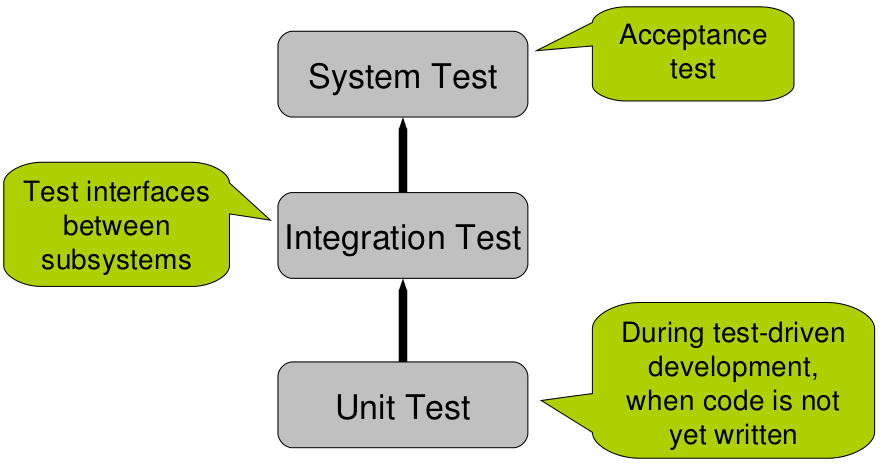
\includegraphics[width=0.5\textwidth]{img/functional_testing.png}
	\item Systematic functional testing
	\\ 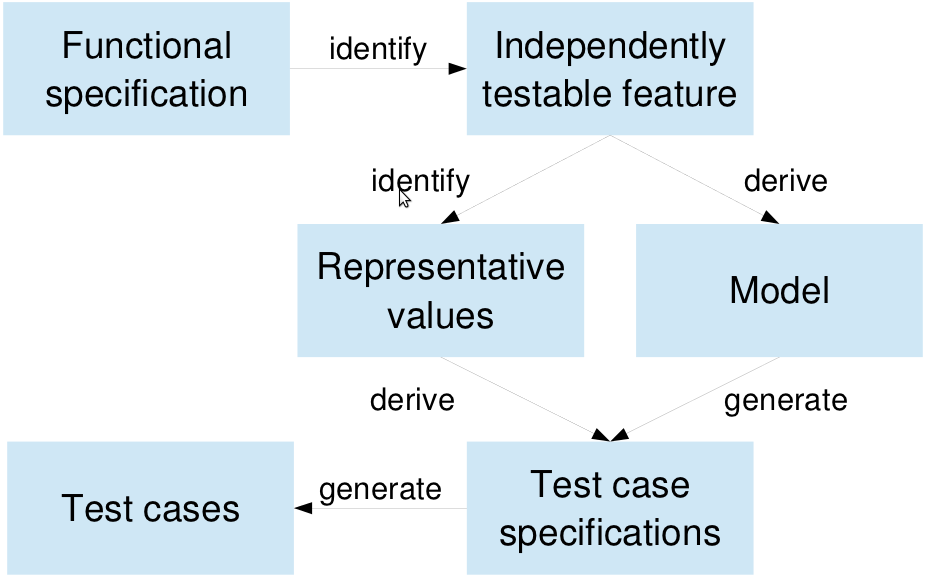
\includegraphics[width=0.5\textwidth]{img/systematic_functional_testing.png}
\enumend

\subsubsection{Functional specification}
\enumstart
	\item Describes technical requirement
	\item not how, but what it does
	\item informal or formal
\enumend

\subsubsection{Independently testable features}
\enumstart
	\item Decompose system into ITF
	\item ITF need not to correspond to classes or subsystems
\enumend

\subsubsection{Identifying representative values}
\enumstart
	\item Divide input into equivalence classes
	\item Chosing representatives for each equivalence class
	\enumstart
		\item Normal values
		\item Invalid values
		\item Special values (e.g. null, empty collection, $\mathellipsis$)
		\item Boundary values (Extreme values inside and outside of boundaries)
	\enumend
\enumend

\subsubsection{Test case specification}
\enumstart
	\item Combine representative values into test data
	\item Combinatorial testing (combine everything) $\rightarrow$ combinatorial explosion
	\enumstart
		\item Use semantic constraints to eliminate combinations
		\item Use domain knowledge to remove unnecessary combinations
	\enumend
	\item Pairwise testing
	\enumstart
		\item Bugs often depend on only a few variables
		\item Test only all pairs of input parameters
		\item Can generalize to $k$-way testing
		\item For $n$ parameters with $d$ values each, number of tests grows log in $n$ and quadratic in $d$
	\enumend
\enumend

\subsubsection{Model-based testing}
\enumstart
	\item Goal: derive test-cases from models
	\item Benefits:
	\enumstart
		\item Compare actual behaviour to modeled behaviour
		\item Measure coverage w.r.t model
		\item (Partly) automate test case generation
	\enumend
	\item Models
	\enumstart
		\item Structural model
		\enumstart
			\item Contains the main concepts manipulated by the system, their properties and relationships
			\item Relevant information
			\enumstart
				\item Classes and attributes
				\item Subtypes
				\item Associations and multiplicities
			\enumend
		\enumend
		\item Behavioral model
		\enumstart
			\item Sequence diagrams (usefull for integration testing)
			\item State diagrams (states $\rightarrow$ equivalence classes)
			\enumstart
				\item State coverage
				\item Transition coverage
			\enumend
		\enumend
		\item Decision structures
		\item Grammars
		\enumstart
			\item Complex inputs can often be described by a (contextfree) grammar
			\item Input of varying and unbounded size
			\item Input with recursive structure
			\item Test cases: Strings generated by the grammar
			\item Coverage criteria
			\enumstart
				\item Production coverage - each production must be used to create a t least one test case
				\item Boundary condition - generate for all productions: Min+1, Min, Max, Max-1
			\enumend
		\enumend
	\enumend
\enumend

\subsection{Structural testing}